\documentclass[11pt]{article}
\usepackage[utf8]{inputenc}
\usepackage{geometry}
\geometry{a4paper}

\usepackage{graphicx}
\usepackage{amsmath,amsthm,amssymb}
\usepackage{amsfonts}
\usepackage{eucal}
\usepackage{gensymb}
\usepackage{yfonts}
\usepackage{epic}
\usepackage{verbatim}
\usepackage{xcolor}
\usepackage{enumitem}
\usepackage{hyperref}
\usepackage{cleveref}
\hypersetup{colorlinks=true,citecolor=blue,linkcolor=blue}
\usepackage{textcomp}
\usepackage{marginnote}
\usepackage{color}
\usepackage{tikz}
\usepackage[font=small,labelfont=bf]{caption}
\usepackage[super]{nth}
\usepackage[framemethod=TikZ]{mdframed}
\mdfdefinestyle{MyFrame}{%
    linecolor=black!75!white,
    outerlinewidth=2pt,
    roundcorner=20pt,
    innertopmargin=\baselineskip,
    innerbottommargin=\baselineskip,
    innerrightmargin=20pt,
    innerleftmargin=20pt,
    backgroundcolor=white}
\definecolor{g3}{gray}{0.9}
\mdfdefinestyle{prob}{%
    linecolor=black!75!white,
    outerlinewidth=2pt,
    roundcorner=5pt,
    %innertopmargin=\baselineskip,
    %innerbottommargin=\baselineskip,
    innerrightmargin=20pt,
    innerleftmargin=20pt,
    backgroundcolor=g3}

\usepackage{fancyhdr}
\usepackage{float}
\usepackage{mdframed}

\usepackage{wrapfig}

\mdfsetup{nobreak=true}

%\oddsidemargin=.2in
%\evensidemargin=.2in
%\topmargin=-.5in
%\textheight=8.5in
%\textwidth=6in

\oddsidemargin=.2in
\evensidemargin=.2in
\topmargin=-.5in
\textheight=8.5in
\textwidth=6in

\usepackage{mathtools}
\DeclarePairedDelimiter{\ceil}{\lceil}{\rceil}

\fancypagestyle{firststyle}{
\fancyhead[L]{
\includegraphics[height=35pt, width= 202 pt, keepaspectratio]{PUMaC_logo_color.png}}
\fancyhead[R]{\includegraphics[height=50pt, width=40 pt]{PU_Shield.png}}}

\fancypagestyle{plain}{
\lhead{PUMaC 2020 Power Round}
\lhead{
\includegraphics[height=17.5pt, width= 101 pt, keepaspectratio]{PUMaC_logo_color.png}}
\rhead{\includegraphics[height=20pt, width=20 pt]{PU_Shield.png}}
\cfoot{}

\crefname{thrm}{}{Theorem}
\crefname{defn}{}{Definiton}

\renewcommand{\headrulewidth}{0.2pt}}
\newcommand{\half}{\frac{1}{2}}
\newcommand{\bbpr}[2]{\mathbb{#1}[#2]}
\newcommand{\E}{\mathbb{E}}
\newcommand{\tr}{\text{tr}}
\newcommand{\aaa}{\text{\textbf{a}}}
\newcommand{\bb}{\text{\textbf{b}}}
\newcommand{\cc}{\text{\textbf{c}}}
\newcommand{\ee}{\text{\textbf{e}}}
\newcommand{\hh}{\text{\textbf{h}}}
\newcommand{\ii}{\text{\textbf{i}}}
\newcommand{\jj}{\text{\textbf{j}}}
\newcommand{\mm}{\text{\textbf{m}}}
\newcommand{\vv}{\text{\textbf{v}}}
\newcommand{\ww}{\text{\textbf{w}}}
\newcommand{\xx}{\text{\textbf{x}}}
\newcommand{\zz}{\text{\textbf{z}}}
\newcommand{\yy}{\text{\textbf{y}}}
\newcommand{\Span}{\text{span}\,}
\newcommand{\C}{\mathbb{C}}
\newcommand{\CC}{\mathcal{C}}
\newcommand{\N}{\mathbb{N}}
\newcommand{\R}{\mathbb{R}}
\newcommand{\Q}{\mathbb{Q}}
\newcommand{\Z}{\mathbb{Z}}
\newcommand{\p}{\mathcal{P}}
\newcommand{\del}{\Delta}
\newcommand{\eps}{\varepsilon}
\newcommand{\sip}[2]{\left\langle#1,#2\right\rangle}
\newcommand{\abs}[1]{\left\lvert#1\right\rvert}
\newcommand{\rhat}{\hat{r}}
\newcommand{\inv}{^{-1}}
\newcommand{\nye}[1]{\tilde{#1}}
\newcommand{\gl}{\mathfrak{gl}}
\newcommand{\Sl}{\mathfrak{sl}}
\newcommand{\Sp}{\mathfrak{sp}}
\newcommand{\So}{\mathfrak{so}}
\newcommand{\ad}{\text{ad}\,}


\newcommand*\sierpinski{\vcenter{\hbox{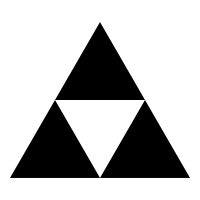
\includegraphics[width=1em]{SierpinskiTriangleIcon.png}}}}



\DeclareMathOperator{\im}{im}

\newtheorem{theorem}[subsubsection]{Theorem}
\newtheorem{lemma}[subsubsection]{Lemma}
\newtheorem{prop}[subsubsection]{Proposition}
\newtheorem{cor}[subsubsection]{Corollary}
\theoremstyle{definition}
\newtheorem{defn}[subsubsection]{Definition}
\newtheorem*{example}{Example}
\theoremstyle{remark}
\newtheorem*{rmk}{Remark}

\newtheoremstyle{problem}{-\topsep}{}{\normalfont}{}{\bfseries}{.}{.5em}{}
\theoremstyle{problem}
\newmdtheoremenv{prob}{Problem}[subsection]
% \newenvironment{prob}{\begin{mdframed}\begin{pro}}
%   {\end{pro}\end{mdframed}}


\title{PUMaC 2024 Power Round: \\ Measures and Fractals}
\author{Colby Riley}
\date{Fall 2024}

\setcounter{section}{0}

\DeclareMathOperator{\Var}{Var}
\DeclareMathOperator{\ex}{ex}

\begin{document}


\thispagestyle{empty}
\noindent \huge{Team Number:} \underline{\phantom{}}

\vspace{.5cm}
\noindent \huge{PUMaC 2024 Power Round Cover Sheet}

\vspace{.5cm}
\normalsize
In years past, this page was for hand-turned in submissions. Now it is for reference for you guys! So that you know how many points each problem is worth. 

\begin{center}
\begin{tabular}{|c|c|c|}\hline
Problem Number & Points & Attempted?\\\hline
2.0.1 & 5 &  \\\hline
2.0.2 & 5 &  \\\hline
2.0.3 & 5 &  \\\hline
2.0.4 & 10 &  \\\hline
2.0.5 & 5 &  \\\hline
2.1.1 & 15 &  \\\hline
2.1.2 & 5 &  \\\hline
2.1.3 & 10 &  \\\hline
2.1.4 & 15 & \\\hline
2.1.5 & 10 & \\\hline
2.1.6 & 5 & \\\hline
2.1.7 & 10 & \\\hline
2.1.8 & 10 & \\\hline
2.1.9 & 5 & \\\hline
4.0.1 & 15 & \\\hline
4.0.2 & 10 & \\\hline
4.0.3 & 15 & \\\hline
4.0.4 & 10 & \\\hline
4.1.1 & 5 & \\\hline
4.1.2 & 5 & \\\hline
4.1.3 & 5 & \\\hline
4.1.4 & 15 & \\\hline
4.1.5 & 10 & \\\hline
\end{tabular}
\hspace{0.5 cm}
\begin{tabular}{|c|c|c|}\hline
Problem Number & Points & Attempted?\\\hline
4.2.1 & 10 & \\\hline
4.2.2 & 10 & \\\hline
4.2.3 & 5 & \\\hline
4.2.4 & 5 & \\\hline
4.2.5 & 20 & \\\hline
4.2.6 & 15 & \\\hline
5.0.1 & 10 & \\\hline
5.0.2 & 5 & \\\hline
5.0.3 & 5 & \\\hline
5.0.4 & 10 & \\\hline
5.0.5 & 25 & \\\hline
5.0.6 & 40 & \\\hline
5.0.7 & 50 & \\\hline
\end{tabular}
\end{center}

\newpage
\tableofcontents
\newpage

\section{Problem 2.0.1}
\textit{Proof:}
\newpage

\section{Problem 2.0.2}
\textit{Proof:}
\newpage

\section{Problem 2.0.3}
\textit{Proof:}
\newpage

\section{Problem 2.0.4}
\textit{Proof:}
\newpage

\section{Problem 2.0.5}
\textit{Proof:}
\newpage

\section{Problem 2.1.1}
\textit{Proof:}
\newpage

\section{Problem 2.1.2}
\textit{Proof:}
\newpage

\section{Problem 2.1.3}
\textit{Proof:}
\newpage

\section{Problem 2.1.4}
\textit{Proof:}
\newpage

\section{Problem 2.1.5}
\textit{Proof:}
\newpage

\section{Problem 2.1.6}
\textit{Proof:}
\newpage

\section{Problem 2.1.7}
\textit{Proof:}
\newpage

\section{Problem 2.1.8}
\textit{Proof:}
\newpage

\section{Problem 2.1.9}
\textit{Proof:}
\newpage

\section{Problem 4.0.1}
\textit{Proof:}
\begin{enumerate}
    \item Let $k = \lceil\log_c(\epsilon/|x-y|)\rceil + 1$ is finite. Notice that 
   \begin{align*}
   |f^{(k)}(x) - f^{(k)}(y)| &= c|f^{(k-1)}(x) - f^{(k-1)}(y)|\\
   &= c^2|f^{(k-2)}(x) - f^{(k-2)}(y)|\\
   &= \cdots\\
   &= c^{k-1}|f(x) - f(y)|\\
   &= c^k |x - y|\\
   &\leq c^{\log_c(\epsilon/|x-y|)+1} |x-y|\\
   &= c\epsilon\\
   &< \epsilon.
   \end{align*}

2. Let $f: \mathbb{R} \to \mathbb{R}$ s.t.
   $$
   f(x) = \frac{x-\sqrt{x^2+4}}{2}.
   $$
    (This is a branch of the hyperbola with $y=x$ and $y=0$ as asymptotes, the branch below both of them.)

   Notice that $f$ is increasing and concave. This is because
   \begin{align*}
   f'(x) &= \frac{1}{2} - \frac{2x}{4\sqrt{x^2+4}}\\
   &= \frac{1}{2} - \frac{x}{2\sqrt{x^2+4}}\\
   &= \frac{\sqrt{x^2+4}-x}{2\sqrt{x^2+4}}\\
   &> \frac{\sqrt{x^2}-x}{2\sqrt{x^2+4}}\\
   &= \frac{|x|-x}{2\sqrt{x^2+4}}\\
   &\geq 0
   \end{align*}
   and so $f'(x)>0$, and
   \begin{align*}
   	f''(x) &= -\frac{1}{2} \cdot \frac{\sqrt{x^2+4} \cdot 1 - x \cdot \frac{1}{2} \cdot 2x \cdot \frac{1}{\sqrt{x^2+4}}}{x^2+4}\\
   	&= -\frac{\sqrt{x^2+4} - \frac{x^2}{\sqrt{x^2+4}}}{2(x^2+4)}\\
   	&= -\frac{(x^2+4) - x^2}{2(x^2+4)\sqrt{x^2+4}}\\
   	&= -\frac{2}{(x^2+4)\sqrt{x^2+4}}\\
   	&< 0,
   \end{align*}
   and so $$f''(x) < 0.$$

   Also, notice that
   \begin{align*}
   	f'(x) - 1 &= \frac{\sqrt{x^2 + 4} -x }{2\sqrt{x^2 + 4}} - 1\\
   	&= - \frac{\sqrt{x^2 + 4} +x }{2\sqrt{x^2 + 4}}\\
   	&<0,
   \end{align*}
   so we can show that $f'(x) < 1$.

   W.L.O.G. let $x > y$, since $f''(y) < 0$, we will know that
   $$
   f(x) - f(y) < (x - y)f'(y) < (x-y)
   $$
   and so $|f(x) - f(y)| < |x-y|$.

   Notice at the same time,
   $$
   f(x) - x = -\frac{x+\sqrt{x^2+4}}{2} < 0
   $$
   so there does not exist $x$ s.t. $f(x) = x$.
\end{enumerate}
\newpage

\section{Problem 4.0.2}
\textit{Proof:} To show that $f(K)$ is compact given $f$ is a contraction and $K$ is compact, we show that $f(K)$ is closed and bounded.

\begin{itemize}
    \item $f(K)$ is bounded: since $K$ is bounded, there exists some $r > 0$ s.t. $K \subset B_{(0, \ldots, 0)} (r)$. In other words, for all $x \in K$, $|x| < r$ .

   Since $f$ is a contraction, set $y = 0$, we will see that $|f(x)| = c|x| < cr$. Therefore, $f(K) \subset B_{(0, \ldots, 0)} (cr)$, which shows $f(K)$ is bounded.
   \item $f(K)$ is closed: since $K$ is closed, $\bar{K}$ is open.
\end{itemize}
\newpage

\section{Problem 4.0.3}
\textit{Proof:}
\newpage

\section{Problem 4.0.4}
\textit{Proof:}
\newpage

\section{Problem 4.1.1}
\textit{Proof:}
\newpage

\section{Problem 4.1.2}
\textit{Proof:}
\newpage

\section{Problem 4.1.3}
\textit{Proof:}
\newpage

\section{Problem 4.1.4}
\textit{Proof:}
\newpage

\section{Problem 4.1.5}
\textit{Proof:}
\newpage

\section{Problem 4.2.1}
\textit{Proof:}
\newpage

\section{Problem 4.2.2}
\textit{Proof:}
\newpage

\section{Problem 4.2.3}
\textit{Proof:}
\newpage

\section{Problem 4.2.4}
\textit{Proof:}
\newpage

\section{Problem 4.2.5}
\textit{Proof:}
\newpage

\section{Problem 4.2.6}
\textit{Proof:}
\newpage

\section{Problem 5.0.1}
\textit{Proof:}
\newpage

\section{Problem 5.0.2}
\textit{Proof:}
\newpage

\section{Problem 5.0.3}
\textit{Proof:}
\newpage

\section{Problem 5.0.4}
\textit{Proof:}
\newpage

\section{Problem 5.0.5}
\textit{Proof:}
\newpage

\section{Problem 5.0.6}
\textit{Proof:}
\newpage

\section{Problem 5.0.7}
\textit{Proof:}
\newpage
\end{document}

